%% LyX 2.3.7 created this file.  For more info, see http://www.lyx.org/.
%% Do not edit unless you really know what you are doing.
\documentclass[10pt,english,t,10pt]{beamer}
\usepackage{lmodern}
\usepackage[T1]{fontenc}
\usepackage[utf8]{inputenc}
\setcounter{tocdepth}{1}
\setlength{\parskip}{\smallskipamount}
\setlength{\parindent}{0pt}
\usepackage{amsbsy}
\usepackage{amstext}
\usepackage[authoryear]{natbib}

\makeatletter
%%%%%%%%%%%%%%%%%%%%%%%%%%%%%% Textclass specific LaTeX commands.
% this default might be overridden by plain title style
\newcommand\makebeamertitle{\frame{\maketitle}}%
% (ERT) argument for the TOC
\AtBeginDocument{%
  \let\origtableofcontents=\tableofcontents
  \def\tableofcontents{\@ifnextchar[{\origtableofcontents}{\gobbletableofcontents}}
  \def\gobbletableofcontents#1{\origtableofcontents}
}

%%%%%%%%%%%%%%%%%%%%%%%%%%%%%% User specified LaTeX commands.



\usepackage{tikz}
\usetikzlibrary{positioning}
\usepackage{appendixnumberbeamer}

\usepackage{graphicx}
\usepackage{subfig}

\usetheme[progressbar=frametitle,block=fill,subsectionpage=progressbar]{metropolis}

% margin
\setbeamersize{text margin right=1.5cm}

% colors
\definecolor{DarkRed}{rgb}{0.7,0,0}
%\colorlet{DarkRed}{red!70!black}
\setbeamercolor{normal text}{fg=black}
\setbeamercolor{alerted text}{fg=DarkRed}
\setbeamercolor{progress bar}{fg=DarkRed}
\setbeamercolor{button}{bg=DarkRed}

% width of seperators
\makeatletter
\setlength{\metropolis@titleseparator@linewidth}{1pt}
\setlength{\metropolis@progressonsectionpage@linewidth}{1pt}
\setlength{\metropolis@progressinheadfoot@linewidth}{1pt}
\makeatother

% new alert block
\newlength\origleftmargini
\setlength\origleftmargini\leftmargini
\setbeamertemplate{itemize/enumerate body begin}{\setlength{\leftmargini}{4mm}}
\let\oldalertblock\alertblock
\let\oldendalertblock\endalertblock
\def\alertblock{\begingroup \setbeamertemplate{itemize/enumerate body begin}{\setlength{\leftmargini}{\origleftmargini}} \oldalertblock}
\def\endalertblock{\oldendalertblock \endgroup}
\setbeamertemplate{mini frame}{}
\setbeamertemplate{mini frame in current section}{}
\setbeamertemplate{mini frame in current subsection}{}
\setbeamercolor{section in head/foot}{fg=normal text.bg, bg=structure.fg}
\setbeamercolor{subsection in head/foot}{fg=normal text.bg, bg=structure.fg}

% footer
\makeatletter
\setbeamertemplate{footline}{%
    \begin{beamercolorbox}[colsep=1.5pt]{upper separation line head}
    \end{beamercolorbox}
    \begin{beamercolorbox}{section in head/foot}
      \vskip1pt\insertsectionnavigationhorizontal{\paperwidth}{}{\hskip0pt plus1filll \insertframenumber{} / \inserttotalframenumber \hskip2pt}\vskip3pt% 
    \end{beamercolorbox}%
    \begin{beamercolorbox}[colsep=1.5pt]{lower separation line head}
    \end{beamercolorbox}
}
\makeatother

% toc
\setbeamertemplate{section in toc}{\hspace*{1em}\inserttocsectionnumber.~\inserttocsection\par}
\setbeamertemplate{subsection in toc}{\hspace*{2em}\inserttocsectionnumber.\inserttocsubsectionnumber.~\inserttocsubsection\par}



% code
\usepackage{xcolor}
\usepackage{listings}

\definecolor{codegray}{rgb}{0.5,0.5,0.5}
\definecolor{background}{HTML}{F5F5F5}
\definecolor{keyword}{HTML}{4B69C6}
\definecolor{string}{HTML}{448C27}
\definecolor{comment}{HTML}{448C27}

\usepackage{inconsolata}
\lstdefinestyle{mystyle}{
    commentstyle=\color{comment},
    keywordstyle=\color{keyword},
    stringstyle=\color{string},
    basicstyle=\ttfamily,
    breakatwhitespace=false,         
    breaklines=true,                 
    captionpos=b,                    
    keepspaces=true,                                    
    numbersep=5pt,                  
    showspaces=false,                
    showstringspaces=false,
    showtabs=false,
    tabsize=4,
	showlines=true
}

\lstset{style=mystyle}

\makeatother

\usepackage{babel}
\begin{document}
\title{14. Advanced HANK Topics\vspace{-2mm}}
\subtitle{Adv. Macro: Heterogenous Agent Models} 
\author{Nicolai Waldstrøm}
\date{2024}

{
\setbeamertemplate{footline}{} 
\begin{frame}

\maketitle

\begin{tikzpicture}[overlay, remember picture]
\node[above left=0cm and 0.0cm of current page.south east] 
{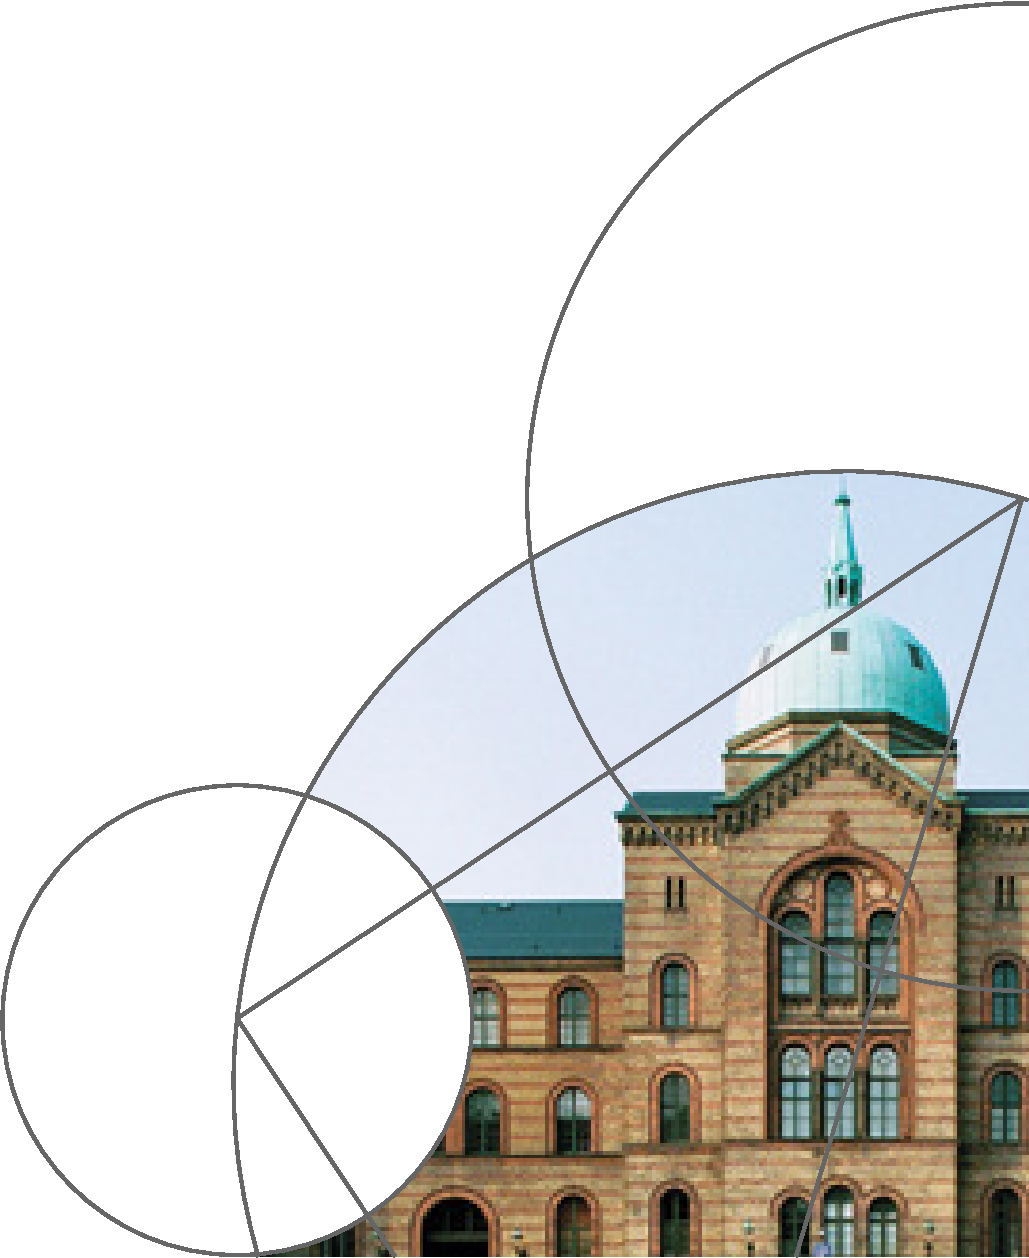
\includegraphics[width=4cm]{figs/KUSAMFtitlelrcorner.pdf}};
\end{tikzpicture}

\begin{tikzpicture}[overlay, remember picture]
\node[below left=0.5cm and .8cm of current page.north east] 
{\includegraphics[width=1.5cm]{figs/KUSAMFlogo.pdf}};
\end{tikzpicture}


\end{frame}
}

\addtocounter{framenumber}{-1}

\section{Introduction}
\begin{frame}{Introduction}
\vspace{-2mm}
\begin{itemize}
\item <+->\textbf{So far:}
\begin{itemize}
\item Utilize HANK framework to study \textbf{how} stabilization policy
(fiscal, monetary) affects the economy
\end{itemize}
\item <+->\textbf{Today: }How does \emph{policy recommendations} change
with the introduction of heterogeneous agents?
\begin{itemize}
\item I.e what is the optimal policy in response to adverse aggregate shocks? 
\item Is it affected by heterogeneity?
\end{itemize}
\item <+->This topic is at the \textbf{research frontier }
\begin{itemize}
\item At the end of lecture I will briefly mention other topics at the frontier
\end{itemize}
\end{itemize}
\end{frame}
%

\section{Optimal Policy}

\begin{frame}{Optimal Policy}
\begin{itemize}
\item <+->What is the problem of the social planner?
\begin{itemize}
\item Consider example where the central bank/social planner chooses the
path of interest rates 
\end{itemize}
\item <+->\textbf{Goal}: Maximize aggregate welfare of \textbf{all} \textbf{households }
\item <+->Subject to:
\begin{itemize}
\item The model (equilibrium conditons, firm + HH behavior, budget constraints
etc)
\item Aggregate shocks 
\end{itemize}
\item <+->This problem is more complicated than calculating \textbf{optimal
steady state policy }
\begin{itemize}
\item <+->Optimal steady state: Maximize one function as a function of
1 or 2 variables (ex: labor income tax+capital income tax)
\item <+->Here: Choose entire \textbf{path} (length T) of instruments subject
to entire dynamic model 
\end{itemize}
\end{itemize}
\end{frame}
%
\begin{frame}{Optimal Policy - computation}
\begin{itemize}
\item <+->Two Approaches:
\end{itemize}
\begin{enumerate}
\item <+->Start from \textbf{efficient} steady state 
\begin{itemize}
\item <+->Harsh assumption
\item <+->No distortions in steady state 
\begin{itemize}
\item No monopolistic competetion, tax distortions
\item No motive for redistribution (i.e. incomplete markets)
\end{itemize}
\item <+->Can then derive quadratic loss function
\item <+->Easy to minimize $\Rightarrow$ Yields optimal Policy
\end{itemize}
\item <+->Start from \textbf{inefficient} steady state 
\begin{itemize}
\item <+->Larger role for inequality and redistribution 
\item <+->Much more difficult - see end of lecture 
\end{itemize}
\end{enumerate}
\end{frame}
%
\begin{frame}{Optimal policy around efficient steady state}
\begin{itemize}
\item <+->Standard NK model features \textbf{inefficient} steady state
due to monopolistic competition 
\item <+->Simple steady state policy can restore efficiency: Give firms
a labor subsidiy $\tau$ such that they charge lower prices 
\item <+->Around\textbf{ efficient steady state}, can derive the following
approximation of household welfare (see e.g. Woodford book):
\[
\mathcal{W}=\sum_{t=0}^{\infty}\beta^{t}\left[u\left(c_{t}\right)-\nu\left(L_{t}\right)\right]\approx-\sum_{t=0}^{\infty}\beta^{t}\left(d\pi_{t}^{2}+\lambda_{Y}dY_{t}^{2}\right)
\]
\item <+->Maximizing welfare same as minizing loss function
\begin{itemize}
\item Planner want to stabilize (varianceof) inflation and output
\end{itemize}
\end{itemize}
\end{frame}
%
\begin{frame}{Solving the planner prob. - efficient steady state}
\begin{itemize}
\item <+->Sequence-space social planner problem ($\boldsymbol{\beta}=\text{diag}\left(1,\beta^{1},\beta^{2},...\right)$):
\[
\min\boldsymbol{\pi}'\boldsymbol{\beta}\boldsymbol{\pi}+\lambda_{Y}d\boldsymbol{Y}'\boldsymbol{\beta}d\boldsymbol{Y}\quad\text{s.t.}\quad H\left(\boldsymbol{Y},\boldsymbol{\pi},\boldsymbol{i},\boldsymbol{\Gamma}\right)=0
\]
\item <+->Stack target variables in vector $\boldsymbol{x}=\left(\boldsymbol{\pi},\boldsymbol{Y}\right)'$
and weights $\boldsymbol{\lambda}=\left(\boldsymbol{1},\lambda_{Y}\right)$.
Then:
\[
\min\boldsymbol{x}'\left(\boldsymbol{\beta}\boldsymbol{\lambda}\right)\boldsymbol{x}\quad\text{s.t.}\quad H\left(\boldsymbol{x},\boldsymbol{i},\boldsymbol{\Gamma}\right)=0
\]
\item <+->Choose interest rate to solve this problem. Solution:
\[
\boldsymbol{i}^{*}=-\left[\boldsymbol{J}_{x,i}'\left(\boldsymbol{\beta}\boldsymbol{\lambda}\right)\boldsymbol{J}_{x,i}\right]^{-1}\times\left[\boldsymbol{J}_{x,i}'\left(\boldsymbol{\beta}\boldsymbol{\lambda}\right)\boldsymbol{J}_{x,\boldsymbol{\Gamma}}d\boldsymbol{\Gamma}\right]
\]
\item <+->\textbf{Easy} to solve for optimal policy given shock $d\boldsymbol{\Gamma}$
- just need jacobians around ss!
\begin{itemize}
\item We need jacobians for $\pi,Y$ w.r.t to the shock $\Gamma$, and the
policy instrument $i$
\end{itemize}
\end{itemize}
\end{frame}
%
\begin{frame}{Interpretation}
\begin{itemize}
\item <+->How to interpret optimal policy formula:
\[
\boldsymbol{i}^{*}=-\left[\boldsymbol{J}_{x,i}'\left(\boldsymbol{\beta}\boldsymbol{\lambda}\right)\boldsymbol{J}_{x,i}\right]^{-1}\times\left[\boldsymbol{J}_{x,i}'\left(\boldsymbol{\beta}\boldsymbol{\lambda}\right)\boldsymbol{J}_{x,\boldsymbol{\Gamma}}d\boldsymbol{\Gamma}\right]
\]
\item <+->Solution to least-squares problem: $\Rightarrow$ Same form as
a OLS least squares estimate (>>$cov\left(\frac{\partial x}{\partial i},\frac{\partial x}{\partial\Gamma}d\boldsymbol{\Gamma}\right)/var\left(\frac{\partial x}{\partial i}\right)$<<)\vspace{0.3cm}
\begin{itemize}
\item If the instrument and the shock co-vary strongly $\Rightarrow$Instrument
is good at offsetting shock, should react more \vspace{0.3cm}
\item If variance of instrument is large (i.e. it has large effects on target
variables) $\Rightarrow$Don't need to change instrument much to get
effect
\end{itemize}
\end{itemize}
\end{frame}
%
\begin{frame}{Optimal policy in HANK - Efficient ss}
\begin{itemize}
\item <+->How does this work in \textbf{HANK}?
\begin{itemize}
\item Main reference: Mckay and Wolf (2022)
\end{itemize}
\item <+->Steady state is \textbf{not efficient }due to incomplete markets
(i.e. borrowing constraint)
\begin{itemize}
\item But need efficient steady state to get quadratic loss function
\end{itemize}
\item <+->Choose general social welfare function (i.e. objective of planner):
\[
\mathcal{W}=\sum_{t=0}^{T}\beta^{t}E_{t}\int\textcolor{red}{\ensuremath{\phi_{j}}}\left[u\left(c_{jt}\right)-\nu\left(L_{t}\right)\right]D_{jt}dj
\]
\item <+->where $\textcolor{red}{\ensuremath{\left\{ \phi_{j}\right\} }}$
is a pareto weight. Mckay and Wolf (2022) calibrate these weights
such that initial steady state efficiente according to objective $\mathcal{W}$
\begin{itemize}
\item If ss features some HHs with low income/wealth with high marginal
utility, then planner will place \textbf{low weight} on these 
\end{itemize}
\end{itemize}
\end{frame}
%
\begin{frame}{Welfare approximation}
\begin{itemize}
\item <+->Given $\textcolor{red}{\ensuremath{\left\{ \phi_{i}\right\} }}$
we can derive a second-order approximation of social welfare:
\begin{alignat*}{1}
\mathcal{W} & =\sum_{t=0}^{T}\beta^{t}E_{t}\int\phi_{j}\left[u\left(c_{jt}\right)-\nu\left(L_{t}\right)\right]D_{jt}dj\\
 & \approx-\sum_{t=0}^{\infty}\beta^{t}\left(d\pi_{t}^{2}+\lambda_{Y}dY_{t}^{2}+\lambda_{\omega}\int\left(d\omega_{jt}\right)^{2}D_{j}dj\right)
\end{alignat*}
\item <+->where $d\omega_{it}\equiv\frac{c_{it}}{C_{t}}-\frac{c_{i,ss}}{C_{ss}}$
is the change in individual $j$'s consumption share
\item <+->Introducing HA give additional motive to social planner to \textbf{stabilize
consumption shares }
\item <+->Implications of inequality for opt. policy depend on distributional
incidence of policy 
\begin{itemize}
\item Heterogeneity matters for monetary policy if this affect cross-sectional
consumption dispersion $\left(\frac{\int\left(d\omega_{jt}\right)^{2}D_{j}dj}{di_{t}}\neq0\right)$
\end{itemize}
\end{itemize}
\end{frame}
%
\begin{frame}{Monetary policy effects}

\begin{itemize}
\item <+->Match model to empirical effects of monetary policy on labor
income + capital gains across wealth distribution:
\item <+->Model implied consumption response across wealth distribution:\\
\begin{figure}[H]     
\centering      
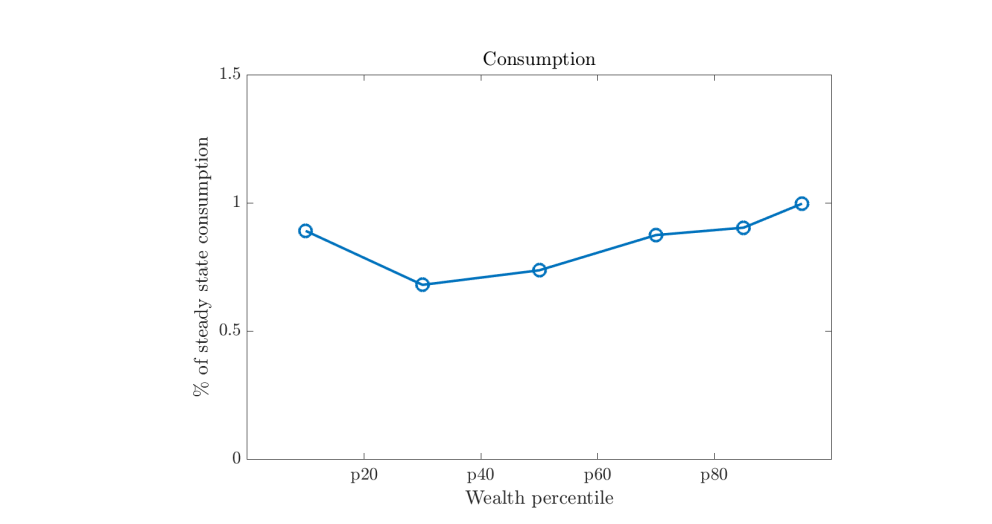
\includegraphics[width=0.7\linewidth]{figs/MW/Fig2MonPolWealth.png}      
\end{figure}
\item <+->Relatively flat - mon. pol. affect $c$ of all HHs proportionally
$\Rightarrow$ consumption shares relatively stable, $\frac{\int\left(d\omega_{jt}\right)^{2}D_{j}dj}{di_{t}}\approx0$
\begin{itemize}
\item {\small{}HHs at bottom of dist. respond to changes in labor income}{\small\par}
\item {\small{}HHs at top of dist. respond (less) to large fluctuations
in cap income (stock prices + house prices)}{\small\par}
\end{itemize}
\end{itemize}
\end{frame}
%
\begin{frame}{Optimal monetary policy - distributional shock}
\begin{itemize}
\item <+->Application: Optimal monetary policy response to \emph{distributional}
shock (transfer from poor to rich)
\begin{itemize}
\item <+->Dual mandate = No inequality term (loss $=-\sum_{t=0}^{\infty}\beta^{t}\left(d\pi_{t}^{2}+\lambda_{Y}dY_{t}^{2}\right)$)
\item <+->Monetary only = Dual mandate + inequality term 
\end{itemize}
\item <+->Inequality term barely affects optimal policy since monetary
policy is ill-suited to offset dist. incidence\\
\begin{figure}[H]     
\centering      
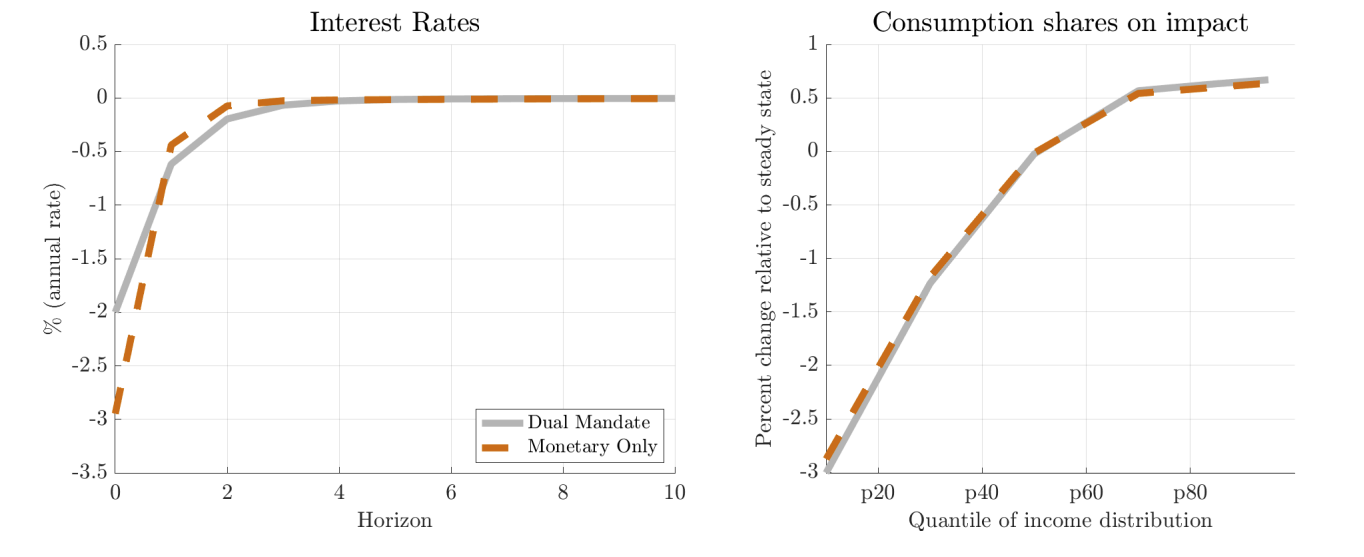
\includegraphics[width=0.7\linewidth]{figs/MW/DistShock.png}      
\end{figure}
\end{itemize}
\end{frame}
%
\begin{frame}{Optimal joint monetary-fiscal policy}
\begin{itemize}
\item <+->If we consider joint monetary \textbf{and} fiscal policy:\\
\begin{figure}[H]     
\centering      
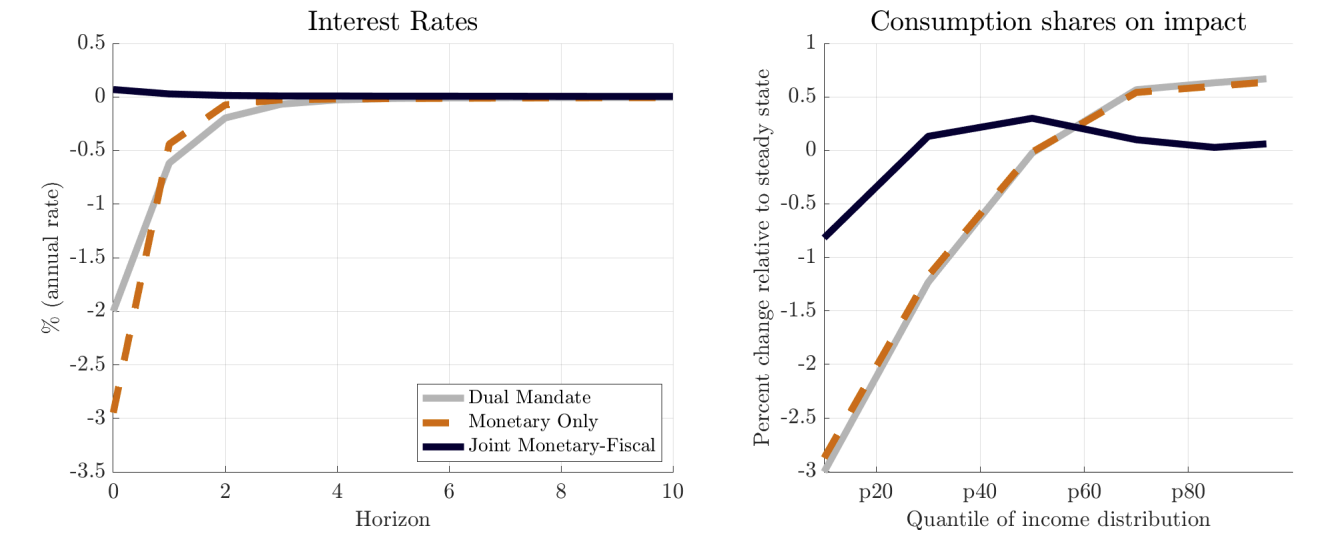
\includegraphics[width=0.7\linewidth]{figs/MW/DistShockJoint.png}      
\end{figure}
\item <+->Fiscal policy good at redistribution - no need for monetary policy
here 
\item <+->Typical sentiment: Fiscal policy should handle redistribution,
not monetar policy
\end{itemize}
\end{frame}
%
\begin{frame}{Quadratic approx: What do we lose?}

\begin{itemize}
\item <+->Mckay-Wolf loss function builds on second-order approximation
of aggregate utility (assume log utility):
\[
\int\phi_{j}u\left(c_{jt}\right)dj\approx u'\left(C\right)\times dC_{t}-\int\frac{\phi_{j}}{c_{j}^{2}}dc_{jt}^{2}dj
\]
\item <+->Weight on variance term $dc_{jt}^{2}$ of individual $j$:
\begin{itemize}
\item Efficient steady state ($\phi_{j}=u'\left(c_{j}\right)^{-1}=c_{j}$):
$1/c_{j}$
\item Infficient steady state and Utilitarian planner ($\phi_{j}=1$): $1/c_{j}^{2}$
\end{itemize}
\item <+->Weights in standard model\\
\begin{figure}[H]     
\centering      
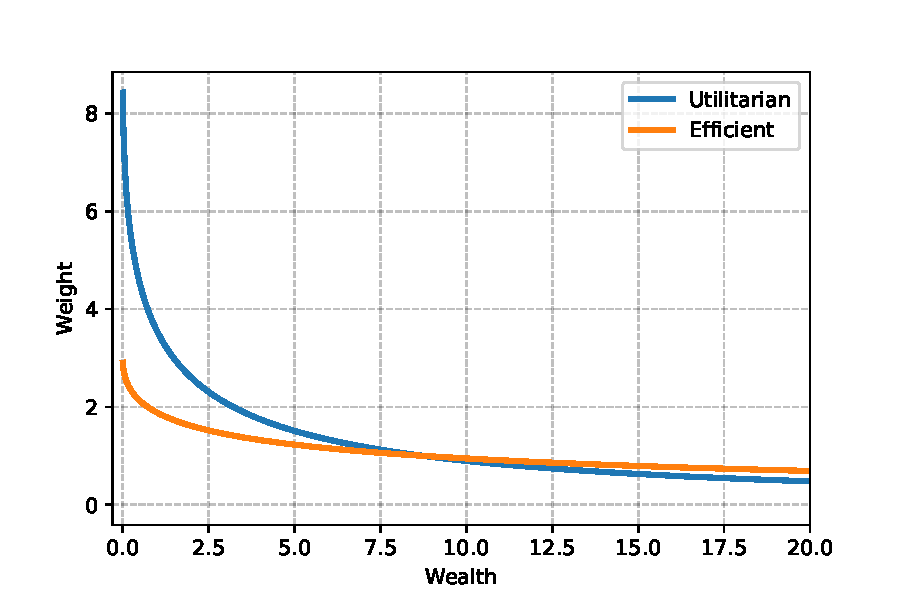
\includegraphics[width=0.5\linewidth]{figs/UtilWeights.pdf}      
\end{figure}
\end{itemize}
\end{frame}
%
\begin{frame}{Optimal Policy from inefficient steady state (Ramsey)}
\begin{itemize}
\item <+->If we do not use use planner weights, HA ss is not efficient
$\Rightarrow$ Cannot derive quad. loss function 
\item <+->\textbf{How to solve for optimal policy?} Example in simple HANK
with optimal monetary policy
\item <+->Simple model with HA, linear production and TFP shock - CB controls
real rate $r$ (\textbf{policy} \textbf{instrument}){\small{}
\begin{alignat*}{1}
\max_{\left\{ r_{t},c_{it},L_{t},Y_{t},w_{t},a_{it}\right\} _{t=0}^{T}}\mathcal{W}= & \sum_{t=0}^{T}\beta^{t}E_{t}\int\left[u\left(c_{it}\right)-\nu\left(L_{t}\right)\right]D_{it}di\\
 & \text{s.t.}\\
c_{it} & =c_{it}^{*}\\
c_{it}+a_{it} & =w_{t}e_{it}+\left(1+r_{t}\right)a_{it-1}\\
Y_{t} & =\Gamma_{t}L_{t}\\
w_{t} & =\Gamma_{t}\\
Y_{t} & =\int c_{it}D_{it}di
\end{alignat*}
}{\small\par}
\end{itemize}
\end{frame}
%
\begin{frame}{Lagrangian I}
\begin{itemize}
\item <+->In Lagrangian form (substitute in and use $w_{t}=\Gamma_{t})$
and $\boldsymbol{x}=\left\{ L_{t}\Gamma_{t},r_{t}\right\} _{t=0}^{T}$
\begin{alignat*}{1}
\mathcal{L}=\max_{\left\{ r_{t},L_{t},\lambda_{t}\right\} _{t=0}^{T}} & \sum_{t=0}^{T}\left\{ \beta^{t}E_{t}\int u\left[\left(c_{it}^{*}\left(\boldsymbol{x}\right)\right)-\nu\left(L_{t}\right)\right]D_{it}\left(\boldsymbol{x}\right)di\right.\\
+ & \left.\lambda_{t}\left[\Gamma_{t}L_{t}-\int c_{it}^{*}\left(\boldsymbol{x}\right)D_{it}\left(\boldsymbol{x}\right)di\right]\right\} 
\end{alignat*}
\item <+->\textbf{FOC} (just w.r.t $r_{s}$):
\begin{alignat*}{1}
\frac{\partial}{\partial r_{s}}\left[\sum_{t=0}^{T}\left\{ \beta^{t}E_{t}\int u\left(c_{it}^{*}\left(\boldsymbol{x}\right)-\nu\left(L_{t}\right)\right)D_{it}di\right.\right]\\
-\frac{\partial}{\partial r_{s}}\sum_{t=0}^{T}\lambda_{t}\int c_{it}^{*}\left(\boldsymbol{x}\right)D_{it}\left(\boldsymbol{x}\right) & di=0
\end{alignat*}
\end{itemize}
\end{frame}
%
\begin{frame}{Lagrangian II}
\begin{itemize}
\item <+->Denote $\boldsymbol{J}^{\mathcal{\mathcal{U}},r}\left(\boldsymbol{x}\right)$
as jacobian of $\mathcal{U}$ w.r.t $r$ evaluated at $\boldsymbol{x}$
\begin{alignat*}{1}
\sum_{t=0}^{T}\beta^{t}\boldsymbol{J}_{t,s}^{\mathcal{\mathcal{U}},r} & \left(\boldsymbol{x}\right)-\sum_{t=0}^{T}\lambda_{t}\boldsymbol{J}_{t,s}^{C,r}\left(\boldsymbol{x}\right)=0
\end{alignat*}
\item <+->First term is (sum) of jacobian of agg. utility $\mathcal{U}$
w.r.t $\boldsymbol{r}$ (gradient)
\item <+->Second term is (sum) of jacobian of agg $\boldsymbol{C}$ w.r.t
$\boldsymbol{r}$ 
\item <+->\textbf{We know how to compute these using fake-news algorithm }
\begin{itemize}
\item We can \textbf{evaluate} the FOCs
\end{itemize}
\end{itemize}
\end{frame}
%
\begin{frame}{Lagrangian FOCs I}
\begin{itemize}
\item <+->Standard techniques (i.e. Fake-news) allow us to evaluate the
following system of FOCs:
\begin{itemize}
\item T eqs. for each (instrument, endogenous variable, lagrange multiplier) 
\end{itemize}
\item <+->How do we \textbf{solve} the system for the optimal policy response?
\item <+->Use (Quasi-)Newton/Broyden's method as usual {[}solve $f\left(x\right)=0$
using $f'\left(x\right)${]}
\item <+->Continue example from before. Jacobian of residual w.r.t $r_{k}$:
\begin{alignat*}{1}
\sum_{t=0}^{T}\beta^{t}\boldsymbol{J}_{t,s}^{\mathcal{\mathcal{U}},r}\left(\boldsymbol{x}\right)-\sum_{t=0}^{T}\lambda_{t}\boldsymbol{J}_{t,s}^{C,r}\left(\boldsymbol{x}\right)=0\\
\Rightarrow\sum_{t=0}^{T}\beta^{t}\frac{\partial\boldsymbol{J}_{t,s}^{\mathcal{\mathcal{U}},r}}{\partial r_{k}}\left(\boldsymbol{x}\right)-\sum_{t=0}^{T}\lambda_{t}\frac{\partial\boldsymbol{J}_{t,s}^{C,r}}{\partial r_{k}}\left(\boldsymbol{x}\right)=0\\
=\sum_{t=0}^{T}\beta^{t}\frac{\partial^{2}\mathcal{\mathcal{U}}_{t}}{\partial r_{s}\partial r_{k}}\left(\boldsymbol{x}\right)-\sum_{t=0}^{T}\lambda_{t}\frac{\partial^{2}C_{t}}{\partial r_{s}\partial r_{k}}\left(\boldsymbol{x}\right)=0
\end{alignat*}
\end{itemize}
\end{frame}
%
\begin{frame}{Lagrangian FOCs II}
\begin{itemize}
\item <+->Last equation repeated:
\[
=\sum_{t=0}^{T}\beta^{t}\frac{\partial^{2}\mathcal{\mathcal{U}}_{t}}{\partial r_{s}\partial r_{k}}\left(\boldsymbol{x}\right)-\sum_{t=0}^{T}\lambda_{t}\frac{\partial^{2}C_{t}}{\partial r_{s}\partial r_{k}}\left(\boldsymbol{x}\right)=0
\]
\item <+->What is the issue here?
\begin{itemize}
\item We need \textbf{\emph{second}} order derivatives to solve this!
\end{itemize}
\item <+->Expensive to get - recall:
\begin{itemize}
\item <+->Jacobian of HH problem requires $T^{2}$ iterations to get for
each input (Fake-news reduce this to $T$)
\item <+->Hessian (size: $T\times T\times T$) requires $T^{3}$ iterations
to get 
\begin{itemize}
\item <+->Can get down to $\frac{T^{2}}{2}$ if we use Fake-news + symmetry
\item <+->Still slow if $T=300$ $\Rightarrow45.000$ evaluations of HH
problem for each input 
\item <+->Getting standard J with Fake-news only requires $T=300$ evaluations 
\end{itemize}
\item <+->Intuition for why this is difficult: the action of every agent
$c_{i},a_{i}$ is a choice variable in the planner's problem $\Rightarrow$
\textbf{massive} max. problem 
\end{itemize}
\end{itemize}
\end{frame}
%
\begin{frame}{Solutions}
\begin{itemize}
\item <+->Bhandari, Evans, Golosov, \& Sargent (2021) 
\begin{itemize}
\item Use small-noise expansions to approximate model w.r.t to both idiosyncratic
states + aggregate shocks 
\item Can handle aggregate uncertainty, but not occ. binding borrowing constraints
\end{itemize}
\item <+->Le Grand \& Ragot (2022)
\begin{itemize}
\item Truncation of state space. Can then derive FOCs by hand
\end{itemize}
\item <+->Dávila \& Schaab (2023)
\begin{itemize}
\item <+->Formulate model in continuous time following Nuño \& Moll (2018)
- can get FOCs of planner problem by hand 
\item <+->Extended to discrete time in Waldstrøm (2024) - use numerical
tools from \emph{deep learning} literature to efficiently compute
derivatives
\end{itemize}
\item Literature not settled - no preferred solution yet!
\end{itemize}
\end{frame}
%

\section{Other HANK Topics }
\begin{frame}{Other HANK topics}
\begin{itemize}
\item <+->Brief introducion to optimal policy in HANK
\item <+->\textbf{Many} other very interesting topics where household heterogeneity
potentially matters
\item <+->I will give you some very brief examples
\begin{itemize}
\item \emph{Could serve as inspiration for master thesis}
\end{itemize}
\end{itemize}
\end{frame}
%
\begin{frame}{Overview}
\begin{itemize}
\item <+->Schaab and Tan (2023) >>Monetary and Fiscal Policy According
to HANK-IO<<
\item <+->Alves \& Violante (2023) >>Some Like It Hot: Monetary Policy
Under Okun’s Hypothesis<<
\item <+->Faccini, Lee, Luetticke, Ravn \& Renkin (2024) >>Financial Frictions:
Macro vs Micro Volatility<< 
\item <+->Ferriere Navarro (2024) >>The heterogeneous effects of government
spending: It’s all about taxes<<
\end{itemize}
\end{frame}
%
\begin{frame}{HANK-IO}
\begin{itemize}
\item <+->Schaab and Tan (2023) >>Monetary and Fiscal Policy According
to HANK-IO<<
\item <+->A multi-sector HANK model where:
\begin{itemize}
\item <+->Households work in different sectors (earnings heterogeneity)
\begin{itemize}
\item May matter for transmission if high MPC HHs work in sectors that are
more cyclical
\end{itemize}
\item <+->Buy goods from sectors (expenditure heterogeneity)
\begin{itemize}
\item May matter for transmission if higher MPC HHs primarily buy goods
from sectors with more flexible prices
\end{itemize}
\end{itemize}
\item <+->Calibrate the model to match these channels using micro data 
\item <+->They find that the contribution of earnings and expenditure heterogeneity
channels in the transmission of monetary policy is small
\end{itemize}
\end{frame}
%
\begin{frame}{Labor Market Dynamics and Monetary Policy}
\begin{itemize}
\item <+->Alves \& Violante (2023) >>Some Like It Hot: Monetary Policy
Under Okun’s Hypothesis<<
\item <+->Poor households are more exposed to business cycles through LM
transition
\begin{itemize}
\item Separation rates + job finding rates are more cyclical
\item Recession have long lasting effects on earnings (recession $\Rightarrow$
leave the LM $\Rightarrow$ hard to get back in)
\end{itemize}
\item <+->\textbf{Trade-off} for CB: Running the economy hot generates
inflaiton (bad) but keeps poor household in labor market (good)
\item <+->Use a HANK model to quantify this trade-off 
\end{itemize}
\end{frame}
%
\begin{frame}{Financial Frictions}
\begin{itemize}
\item <+->Faccini, Lee, Luetticke, Ravn \& Renkin (2024) >>Financial Frictions:
Macro vs Micro Volatility<< 
\item <+->Borrowers and savers pay different interest rates 
\item <+->The spread (interest on loans minus savings) is countercyclical 
\begin{itemize}
\item <+->A monetary policy shock that increases the interbank rate causes
banks to raise rates on loans more than on savings 
\item <+->This reduces the mass of household at $a<0$ who move to $a=0$
through deleveraging
\end{itemize}
\item <+->The aggregate MPCs increases by up to 5\% in \textbf{response}
to a monetary policy shock due to this mechanism 
\end{itemize}
\end{frame}
%
\begin{frame}{Progressive Taxes}
\begin{itemize}
\item <+->Ferriere \& Navarro (2024) >>The heterogeneous effects of government
spending: It’s all about taxes<<
\begin{itemize}
\item Uncover \emph{Progressivity-dependent fiscal multipliers}
\end{itemize}
\item <+->Observation: Low income households:
\begin{itemize}
\item 1) Have higher MPCs 
\item 2) Have larger labor supply elasticities 
\end{itemize}
\item <+->Result: Government spending shocks which are financed by more
progressive taxes have higher multipliers
\item <+->Consistent with empirical evidence
\end{itemize}
\end{frame}
%

\section{Conclusion}
\begin{frame}{Conclusion}
\begin{itemize}
\item \textbf{Today: }
\begin{itemize}
\item A brief look into current research frontier on HANK 
\item \textbf{Many} other papers which we have not covered
\end{itemize}
\item \textbf{Now: }Exam\textbf{ }
\end{itemize}
\end{frame}
%

\end{document}
